\documentclass[tikz, border=5mm]{standalone}
\usepackage{amsmath}
\usepackage{amssymb}
\usetikzlibrary{calc, arrows.meta, shapes.geometric, positioning, decorations.pathreplacing}

\begin{document}
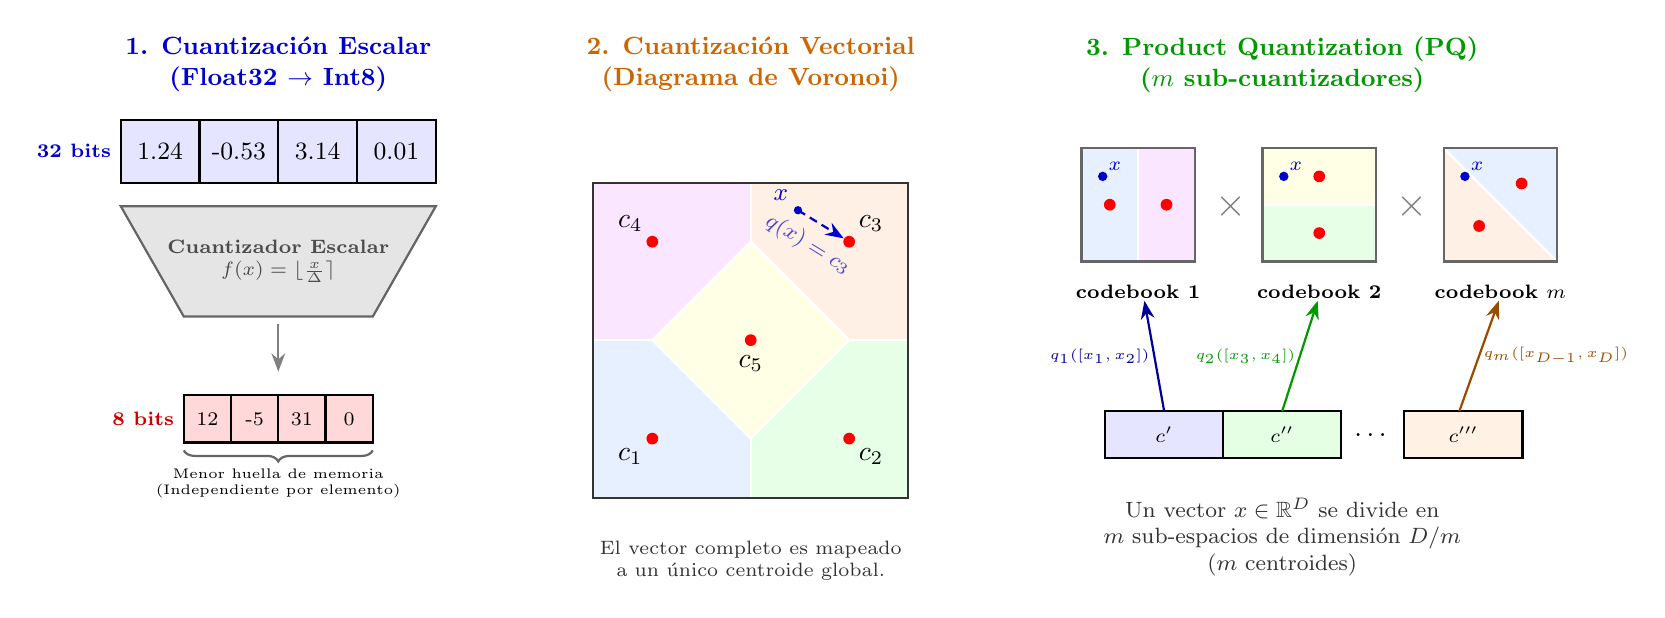
\begin{tikzpicture}[
    % Estilos globales
    title style/.style={font=\bfseries\small, align=center},
    arrow line/.style={->, >=Stealth, thick, color=black!60},
    centroid/.style={circle, fill=red, inner sep=1.5pt},
    vq arrow/.style={->, >=Stealth, thick, blue!80!black, densely dashed}
]

    % Definición de colores pastel para Voronoi
    \definecolor{cell1}{RGB}{230, 240, 255}
    \definecolor{cell2}{RGB}{230, 255, 230}
    \definecolor{cell3}{RGB}{255, 240, 230}
    \definecolor{cell4}{RGB}{250, 230, 255}
    \definecolor{cell5}{RGB}{255, 255, 230}

    % =========================================================================
    % CUADRO 1 (Izquierda): Cuantización Escalar (SQ)
    % =========================================================================
    \begin{scope}[xshift=0cm, yshift=0cm]
        % Marco
        %\draw[draw=black!20, fill=gray!5, rounded corners] (-0.5, -1) rectangle (4.5, 6.5);
        \node[title style, color=blue!80!black] at (2.0, 6.0) {1. Cuantización Escalar\\(Float32 $\rightarrow$ Int8)};

        % 1. Vector Original (Float32) - Bloques grandes
        \begin{scope}[yshift=4.5cm, xshift=0cm]
            \foreach \i/\val in {0/1.24, 1/-0.53, 2/3.14, 3/0.01} {
                \draw[fill=blue!10, thick] (\i, 0) rectangle (\i+1, 0.8) node[midway, font=\small] {\val};
            }
            \node[left, font=\scriptsize\bfseries, color=blue!80!black] at (0, 0.4) {32 bits};
        \end{scope}

        % 2. Embudo (Funnel) de compresión
        \draw[fill=gray!20, thick, draw=black!60] 
            (0, 4.2) -- (4, 4.2) -- (3.2, 2.8) -- (0.8, 2.8) -- cycle;
        
        \node[align=center, font=\scriptsize\bfseries, color=black!70] at (2.0, 3.5) {Cuantizador Escalar\\$f(x) = \lfloor \frac{x}{\Delta} \rceil$};
        \draw[->, >=Stealth, thick, black!50] (2.0, 2.7) -- (2.0, 2.1);

        % 3. Vector Cuantizado (Int8) - Bloques comprimidos y empaquetados
        \begin{scope}[yshift=1.2cm, xshift=0.8cm]
            % Los bloques son más estrechos para ilustrar la reducción de tamaño
            \foreach \i/\val in {0/12, 1/-5, 2/31, 3/0} {
                \draw[fill=red!15, thick] (\i*0.6, 0) rectangle (\i*0.6 + 0.6, 0.6) node[midway, font=\scriptsize] {\val};
            }
            \node[left, font=\scriptsize\bfseries, color=red!80!black] at (0, 0.3) {8 bits};
        \end{scope}
        
        % Llave indicando empaquetamiento en memoria
        \draw[decorate, decoration={brace, amplitude=4pt, mirror}, thick, black!60] 
            (0.8, 1.1) -- (3.2, 1.1) node [black, midway, yshift=-12pt, font=\tiny, align=center] {Menor huella de memoria\\(Independiente por elemento)};
    \end{scope}

    % =========================================================================
    % CUADRO 2 (Centro): Cuantización Vectorial (VQ / Voronoi)
    % =========================================================================
    \begin{scope}[xshift=5.5cm, yshift=0cm]
        % Marco
        %\draw[draw=black!20, fill=gray!5, rounded corners] (-0.5, -1) rectangle (5.5, 6.5);
        \node[title style, color=orange!80!black] at (2.5, 6.0) {2. Cuantización Vectorial\\(Diagrama de Voronoi)};

        % Escalar el diagrama de Voronoi anterior para que quepa en el panel
        \begin{scope}[shift={(0.5, 0.5)}, scale=0.5]
            
            % Polígonos de celdas
            \fill[cell1] (0,0) -- (4,0) -- (4,1.5) -- (1.5,4) -- (0,4) -- cycle;
            \fill[cell2] (4,0) -- (8,0) -- (8,4) -- (6.5,4) -- (4,1.5) -- cycle;
            \fill[cell3] (8,4) -- (8,8) -- (4,8) -- (4,6.5) -- (6.5,4) -- cycle;
            \fill[cell4] (0,4) -- (1.5,4) -- (4,6.5) -- (4,8) -- (0,8) -- cycle;
            \fill[cell5] (4,1.5) -- (6.5,4) -- (4,6.5) -- (1.5,4) -- cycle;

            % Fronteras
            \draw[thick, white] (4,0) -- (4,1.5);
            \draw[thick, white] (8,4) -- (6.5,4);
            \draw[thick, white] (4,8) -- (4,6.5);
            \draw[thick, white] (0,4) -- (1.5,4);
            \draw[thick, white] (4,1.5) -- (6.5,4) -- (4,6.5) -- (1.5,4) -- cycle;
            \draw[thick, black!80] (0,0) rectangle (8,8);

            % Centroides
            \node[centroid] (c1) at (1.5, 1.5) {}; \node[below left, font=\bfseries] at (c1) {$c_1$};
            \node[centroid] (c2) at (6.5, 1.5) {}; \node[below right, font=\bfseries] at (c2) {$c_2$};
            \node[centroid] (c3) at (6.5, 6.5) {}; \node[above right, font=\bfseries] at (c3) {$c_3$};
            \node[centroid] (c4) at (1.5, 6.5) {}; \node[above left, font=\bfseries] at (c4) {$c_4$};
            \node[centroid] (c5) at (4, 4) {};     \node[below=2pt, font=\bfseries] at (c5) {$c_5$};

            % Vector x mapeado
            \coordinate (X) at (5.2, 7.3);
            \fill[blue!80!black] (X) circle (3pt) node[above left, font=\small] {$x$};
            \draw[vq arrow] (X) -- (c3) node[midway, sloped, above=-14pt, font=\footnotesize, fill=cell3, fill opacity=0.7, inner sep=1pt] {$q(x) = c_3$};
        \end{scope}

        % Leyenda inferior
        \node[font=\scriptsize, align=center, black!80] at (2.5, -0.3) {El vector completo es mapeado\\a un único centroide global.};
    \end{scope}

    % =========================================================================
    % CUADRO 3 (Derecha): Product Quantization (PQ)
    % =========================================================================
    \begin{scope}[xshift=12cm, yshift=0cm]
        % Marco
        %\draw[draw=black!20, fill=gray!5, rounded corners] (-0.5, -1) rectangle (6.0, 6.5);
        \node[title style, color=green!60!black] at (2.75, 6.0) {3. Product Quantization (PQ)\\($m$ sub-cuantizadores)};

        % --- Parte Superior: Subespacios de Voronoi Superpuestos ---
        % Sub-cuantizador 1
        \begin{scope}[shift={(0.2, 3.5)}, scale=0.18]
            \fill[cell1] (0,0) rectangle (4,8); \fill[cell4] (4,0) rectangle (8,8);
            \draw[thick, white] (4,0) -- (4,8); \draw[thick, black!60] (0,0) rectangle (8,8);
            \node[centroid] at (2,4) {}; \node[centroid] at (6,4) {};
            \node[below, font=\scriptsize\bfseries] at (4, -1) {codebook 1};

            \node[circle, fill=blue!80!black, inner sep=1.2pt] (x1) at (1.5, 6) {};
            \node[above right=-2pt, font=\scriptsize, text=blue!80!black] at (x1) {$x$};
        \end{scope}
        
        \node[font=\bfseries\Large, black!50] at (2.1, 4.2) {$\times$};

        % Sub-cuantizador 2
        \begin{scope}[shift={(2.5, 3.5)}, scale=0.18]
            \fill[cell2] (0,0) rectangle (8,4); \fill[cell5] (0,4) rectangle (8,8);
            \draw[thick, white] (0,4) -- (8,4); \draw[thick, black!60] (0,0) rectangle (8,8);
            \node[centroid] at (4,2) {}; \node[centroid] at (4,6) {};
            \node[below, font=\scriptsize\bfseries] at (4, -1) {codebook 2};

            \node[circle, fill=blue!80!black, inner sep=1.2pt] (x1) at (1.5, 6) {};
            \node[above right=-2pt, font=\scriptsize, text=blue!80!black] at (x1) {$x$};
        \end{scope}

        \node[font=\bfseries\Large, black!50] at (4.4, 4.2) {$\times$};

        % Sub-cuantizador m (3)
        \begin{scope}[shift={(4.8, 3.5)}, scale=0.18]
            \fill[cell3] (0,0) -- (8,0) -- (0,8) -- cycle; \fill[cell1] (8,8) -- (0,8) -- (8,0) -- cycle;
            \draw[thick, white] (0,8) -- (8,0); \draw[thick, black!60] (0,0) rectangle (8,8);
            \node[centroid] at (2.5,2.5) {}; \node[centroid] at (5.5,5.5) {};
            \node[below, font=\scriptsize\bfseries] at (4, -1) {codebook $m$};

            \node[circle, fill=blue!80!black, inner sep=1.2pt] (x1) at (1.5, 6) {};
            \node[above right=-2pt, font=\scriptsize, text=blue!80!black] at (x1) {$x$};
        \end{scope}

        % --- Parte Inferior: División del Vector en Bloques ---
        \node[font=\footnotesize, align=center, black!80] at (2.75, 0.0) {Un vector $x \in \mathbb{R}^D$ se divide en\\$m$ sub-espacios de dimensión $D/m$ \\ ($m$ centroides)};

        % Dibujo del vector largo dividido
        \begin{scope}[yshift=1.0cm, xshift=0.5cm]
            % Bloque 1
            \draw[fill=blue!10, thick] (0, 0) rectangle (1.5, 0.6) node[midway, font=\scriptsize] {$c'$};
            % Bloque 2
            \draw[fill=green!10, thick] (1.5, 0) rectangle (3.0, 0.6) node[midway, font=\scriptsize] {$c''$};
            % Puntos suspensivos para indicar generalización
            \node at (3.4, 0.3) {$\dots$};
            % Bloque m
            \draw[fill=orange!10, thick] (3.8, 0) rectangle (5.3, 0.6) node[midway, font=\scriptsize] {$c'''$};
        \end{scope}

        % Flechas conectando los bloques del vector a sus respectivos subespacios
        \draw[arrow line, blue!60!black] (1.25, 1.6) -- (1.0, 3.0) node[midway, left=-2pt, font=\tiny] {$q_1([x_1, x_2])$};
        \draw[arrow line, green!60!black] (2.75, 1.6) -- (3.2, 3.0) node[midway, left=-2pt, font=\tiny] {$q_2([x_3, x_4])$};
        \draw[arrow line, orange!60!black] (5.0, 1.6) -- (5.5, 3.0) node[midway, right=-2pt, font=\tiny] {$q_m([x_{D-1}, x_{D}])$};

    \end{scope}


\end{tikzpicture}
\end{document}
